\documentclass{article}
\usepackage{my_style}
\usepackage{environ}
\usepackage[font=scriptsize]{caption}
\begin{document}

\vspace*{3cm}
\thispagestyle{empty}
\begin{center}
    {\huge \textbf{Simulación de Asistencia Gravitatoria}}\\
    \vspace*{1cm}
    {\LARGE Íñigo Aliod López}

    \vspace*{.5cm}

    {\large Mecánica Clásica I}
\end{center}
\vspace*{4cm}

% \begin{figure}[h]
%     \centering
%     \resizebox{1\textwidth}{!}
%     {\includegraphics{figuras/portada/portada.pdf}}
% \end{figure}

% \newpage

\begin{abstract}
\noindent En el presente trabajo se explora la optimización de una maniobra de asistencia gravitatoria, un problema central en la mecánica celeste, mediante la creación de un simulador N-cuerpos en C. Utilizando un integrador Runge-Kutta de cuarto orden con paso adaptativo, y orquestando barridos de parámetros con Python, se ha buscado sistemáticamente la dirección de lanzamiento óptima para una sonda inspirada en la misión Solar Orbiter. El análisis ha revelado la existencia de dos familias de trayectorias óptimas; una que resulta en una pérdida de energía de la nave, cumpliendo el objetivo de acercarse al Sol, y otra, que provoca una ganancia energética. Se concluye que la metodología de barrido en múltiples fases es una herramienta eficaz para la optimización de trayectorias interplanetarias, validando los resultados con un análisis riguroso de la conservación de la energía del sistema.
\end{abstract}

\newpage
\tableofcontents

\section{Introducción y marco teórico}
Este trabajo aspira a simular el Sistema Solar con datos realistas, para lograr recrear una 
maniobra de asistencia gravtitatoria, 
con datos y trayectoria similares a los de la nave \textbf{Solar Orbiter} de la Agencia Espacial Europea (ESA).

Una asistencia gravitatoria consiste en el intercambio de energía, por medio de la variación del momento angular, 
entre un cuerpo celeste y una nave.
El objetivo del presente trabajo es intentar maximizar dicho intercambio de energía (que tendrá que ser negativo) 
para acercarse lo 
máximo posible al Sol.

\subsection{Parámetros iniciales}
Los parámetros físicos fundamentales utilizados en la simulación han sido extraídos de fuentes oficiales para 
garantizar la precisión de los resultados. De la base de datos del \textit{Jet Propulsion Laboratory} (JPL) de 
la NASA\footnote{\texttt{https://ssd.jpl.nasa.gov/astro\_par.html}}, han sido extraídos el valor de la 
constante de gravitación universal $G$ y los 
parámetros gravitacionales estandarizados de los distintos cuerpos. Dado que estos sistemas proporcionan 
las masas en la forma del parámetro gravitacional $G M$, las masas individuales,
$M_\circ$, $M_T$, $M_J$, $M_m$, $M_v$, han sido obtenidas dividiendo los valores por $G$. 
Para ciertos parámetros orbitales específicos 
y radios, como los de la Luna, se han consultado fuentes como la \textit{Planetary Fact Sheet} de la 
NASA\footnote{\texttt{http://www.mathaddict.net/ellipseplanet.pdf}} y 
tablas de mecánica celeste estandarizadas\footnote{\texttt{https://www.mnealon.eosc.edu/NewtonianMechanics.htm}}.

Así, utilizando los datos aportados por el sistema \textit{Horizons} del JPL de la NASA, es posible simular 
los planetas en su posición real el día en el que se lanzó el \textit{Solar Orbiter}. Dado que las coordenadas 
de la nave no están disponibles en el momento exacto de lanzamiento (pues está en la Tierra), se toman las 
coordenadas de los planetas a las 00:00 del 11 de febrero de 2020, unas 20 horas después del lanzamiento.

\subsection{Condiciones iniciales de la nave}
Para obtener unas condiciones iniciales realistas para la nave, se recurre de nuevo al sistema 
\textit{Horizons} del JPL de la NASA para extraer tanto el vector de posición como el vector de velocidad 
del \textit{Solar Orbiter} en ese instante, a las 00:00 del 11 de febrero de 2020. 

% Al transcurrir este tiempo desde el lanzamiento, la sonda ya ha establecido su trayectoria de 
% transferencia interplanetaria inicial, alejándose de la Tierra para escapar de su Esfera de Influencia, 
% situándose a una distancia que aproximaremos a $\frac{49}{50}$ UA respecto a la posición original, 
% o unos 3 millones de kilómetros, donde la perturbación gravitatoria terrestre es ya residual y 
% no domina la dinámica orbital en favor del Sol.

Esto permite fijar un módulo de velocidad inicial y una posición de partida que son físicamente realistas 
y coherentes con la capacidad de los lanzadores de la misión real; sin embargo, si se utilizara 
también la dirección exacta del vector velocidad proporcionado por el JPL, el trabajo quedaría reducido a una mera 
recreación de la trayectoria histórica. 
Debido a ello, dicha dirección será obviada y se planteará un problema de optimización:
encontrar la dirección de lanzamiento óptima que minimice la distancia de aproximación a Venus para así maximizar
la transferencia de energía entre el planeta y la nave.

\subsubsection{Justificación Analítica de la Asistencia Gravitatoria}
La relación entre la distancia de aproximación (periapsis, $r_p$) y el intercambio de energía se puede justificar analíticamente. 
En el sistema de referencia planetario, la nave describe una trayectoria hiperbólica, 
que no es más que la solución matemática de un problema de dispersión gravitatoria.
Es análogo a la dispersión de Rutherford, siendo la única diferencia que tratamos con un potencial atrctivo en vez de repulsivo
(potencial $V(r) \propto +1/r$ en vez de $V(r) \propto -1/r$).
Esto resulta en un cambio de signo en la ecuación de la trayectoria, siendo la de la atractiva:
$$r = \frac{p}{1 + \varepsilon\cos \beta}$$
Sin embargo, la relación final entre el ángulo de 
dispersión $\theta$ y la excentricidad se mantiene idéntica en ambos casos:
$$\sin\left(\frac{\theta}{2}\right) = \frac{1}{\varepsilon}$$

\paragraph{Excentricidad en función de la periapsis.}
La excentricidad de una órbita en un campo de fuerzas centrales con potencial $V = -k/r$ viene dada por la expresión general:
\begin{equation}
    \varepsilon = \sqrt{1 + \frac{2 E J^2}{m k^2}}
\end{equation}
donde $E$ es la energía mecánica total, $J$ el momento angular total y $m$ la masa de la nave. Para el potencial gravitatorio, el factor $k$ es $k = G M_V m$, donde $M_V$ es la masa de Venus.
\newpage
Sustituyendo $k$ y las expresiones para la energía lejos del planeta ($E = \frac{1}{2}mv_\infty^2$) y el momento angular al cuadrado ($J^2 = m^2(r_p^2 v_\infty^2 + 2 G M_V r_p)$), obtenemos:
\begin{equation}
    \varepsilon^2 = 1 + \frac{2 \left(\frac{1}{2}mv_\infty^2\right) \left(m^2(r_p^2 v_\infty^2 + 2 G M_V r_p)\right)}{m(m G M_V)^2}
\end{equation}
Simplificando los términos de masa $m$:
\begin{align}
    \varepsilon^2 &= 1 + \frac{m^3 v_\infty^2 (r_p^2 v_\infty^2 + 2 G M_V r_p)}{m^3 (G M_V)^2} \nonumber \\
    &= 1 + \frac{v_\infty^2 (r_p^2 v_\infty^2 + 2 G M_V r_p)}{(G M_V)^2} \nonumber \\
    &= 1 + \frac{r_p^2 v_\infty^4}{(G M_V)^2} + \frac{2 r_p v_\infty^2}{G M_V} = \left(1 + \frac{r_p v_\infty^2}{G M_V}\right)^2
\end{align}
De donde se obtiene la relación fundamental, que es independiente de la masa de la nave ($m$):
\begin{equation}
    \varepsilon = 1 + \frac{r_p v_\infty^2}{G M_V}
\end{equation}

\paragraph{Ángulo de giro y cambio de velocidad.}
Al sustituir la expresión de $\epsilon$ en la ecuación 1, se obtiene la primera fórmula clave:
\begin{equation}
    \sin\left(\frac{\theta}{2}\right) = \frac{1}{1 + \dfrac{r_p v_\infty^2}{G M_V}}
\end{equation}
El cambio de velocidad, $\Delta v$, se obtiene por geometría vectorial. 
Dado que la energía se conserva, el módulo de la velocidad de entrada y de salida es el mismo ($v_\infty$). 
El vector $\Delta \vec{v}$ forma la base de un triángulo isósceles, cuyo módulo es 
$\Delta v = 2 v_\infty \sin(\theta/2)$. Combinando ambas ecuaciones, se obtiene la expresión final:
\begin{equation}
    \Delta v = \frac{2 v_\infty}{1 + \dfrac{r_p v_\infty^2}{G M_V}}
\end{equation}
Como se observa, para maximizar el cambioo de velocidad $\Delta v$ y maximizar la transferencia 
energética, se debe minimizar la distancia de periapsis $r_p$.
Sin embargo, esta optimización cuenta con una restricción física indispensable: 
para que la sonda pueda continuar su misión, no debe colisionar con la superficie de Venus 
ni desintegrarse por la fricción aerodinámica con la atmósfera (ni perder energía por esta). 
\newpage
Por tanto, la distancia mínima de aproximación debe cumplir siempre la condición límite de que 
$r_p > R_V + h_{\text{atm}}$, siendo $R_V$ el radio del planeta y $h_{\text{atm}}$ el 
límite superior de su atmósfera.
Añadiremos, además, una holgura extra para evitar cualquier tipo de pérdida energética por un posible
rozamiento con la atmósfera; el radio de Venus es de 6052km según las fuentes  
nombradas anteriormente, y su exosfera se encuentra a 350km.

Además, aunque el Sistema Solar interior es fundamentalmente coplanario, las órbitas presentan ligeras inclinaciones respecto a otras; 
en nuestro caso concreto, la órbita de Venus tiene una inclinación de aproximadamente $3.4^\circ$ respecto a la eclíptica. 
Si cada simulación estuviera limitara a un único grado de libertad variando solo el ángulo de guiñada, $\varphi$,
la nave quedaría contenida en el mismo plano para todas las simulaciones.

Debido a esto, se realizará un barrido sobre dos grados de libertad: el ángulo de guiñada (yaw), $\varphi$, y el de cabeceo
(pitch), $\theta$.
El hecho de mantener fijo el módulo de la velocidad a uno realista, permite acotar el coste computacional de las simulaciones,
y restringir el mapa de soluciones a uno bidimensional, facilitando así su interpretación.
\section{Simulaciones y barrido del espacio de parámetros}
Para lograr un equilibrio entre coste computacional y precisión, se ha optado por utilizar
el algoritmo de Runge-Kutta de cuarto orden (RK4), implementando un paso de 
tiempo adaptativo, gobernado por los siguientes parámetros:
\begin{itemize}
    \item \texttt{total\_t}: El tiempo total de simulación.
    Este periodo debe ser suficiente para abarcar toda la trayectoria de transferencia desde el lanzamiento 
    hasta un posible encuentro con Venus.
    \item \texttt{factor}, $f$: Factor de tolerancia multiplicativo. 
    Este parámetro se fija de manera arbitraria, y multiplicará a la fórmula del cáclulo de $dt$.
    \item \texttt{precision\_factor}, $p_f$: Factor divisor de precisión. 
    Cuando la nave se acerque a una distancia crítica, que se ha fijado
    de forma completamente arbitraria en $10^6\text{ km}$, el paso temporal $dt$ se divide por 
    este factor para simular correctamente la violenta variación de energía sufrida en la asistencia gravitatoria
    \footnote{Esto supone una pequeña discontinuidad en la energía, lo que se ve reflejado en las gráficas
    de energía; sin embargo, esta variación es del orden de magnitud de la variación total a lo largo de toda la simulación;
    del orden de $10^{-14}$}.
    \item \texttt{max\_dt}, $M_{dt}$, y \texttt{min\_dt}, $m_{dt}$: Los topes superior e 
    inferior del paso de tiempo (expresados en segundos). Permiten que la simulación 
    avance rápidamente cuando no es necesaria una precisión extrema, y evitan que la simulación 
    quede bloqueada intentando conseguir una precisión infinita cuando la distancia es muy pequeña.
\end{itemize}
Con todo, el valor de \texttt{dt} se calculará utilizando la siguiente expresión:
$$
dt = f \cdot \sqrt[3]{r_v}
$$
Donde $r_v$ es la distancia a Venus de la nave.
Además, nos podemos encontrar con las siguientes casuísticas:
Además, se pueden encontrar las siguientes casuísticas:
\begin{itemize}
    \item Si $dt > M_{dt}$, se asigna $dt = M_{dt}$.
    \item Si $dt < m_{dt}$, se asigna $dt = m_{dt}$.
    \item Si $r_v < 10^9\text{ m}$, se asigna $dt = \dfrac{dt}{p_f}$ (es decir, se divide por \texttt{precision\_factor}).
\end{itemize}

\subsection{Primera aproximación}
En primer lugar, con el objetivo de realizar una exploración inicial del espacio de parámetros, 
se ha planteado un barrido grueso de 65341 simulaciones, para barrer el espacio cada $1^\circ$ de cada grado de libertad. 
Dado el elevado número de ejecuciones, se ha optado por relajar la precisión del integrador numérico para acelerar 
los cálculos, pero sin comprometer significativamente la validez física del sistema.
De este modo, los parámetros de inicialización del código utilizados para esta primera aproximación son:

\bigskip
\noindent\begin{minipage}{0.5\textwidth}\scriptsize
\begin{verbatim}
double min_yaw_angle = -180.0;
double max_yaw_angle = 180.0;
double min_pitch_angle = -90.0;
double max_pitch_angle = 90.0;
double total_t = 400.0;
double factor = 0.1;
\end{verbatim}
\end{minipage}%
\begin{minipage}{0.5\textwidth}\scriptsize
\begin{verbatim}
double precision_factor = 10.0;
double max_dt = 100;
double min_dt = 0.1;
int pitch_sims = 181;
int yaw_sims = 361;
int total_sims = yaw_sims*pitch_sims;
\end{verbatim}
\end{minipage}

\bigskip

Se obtiene así el siguiente gráfico:
\begin{figure}[H]
    \centering
    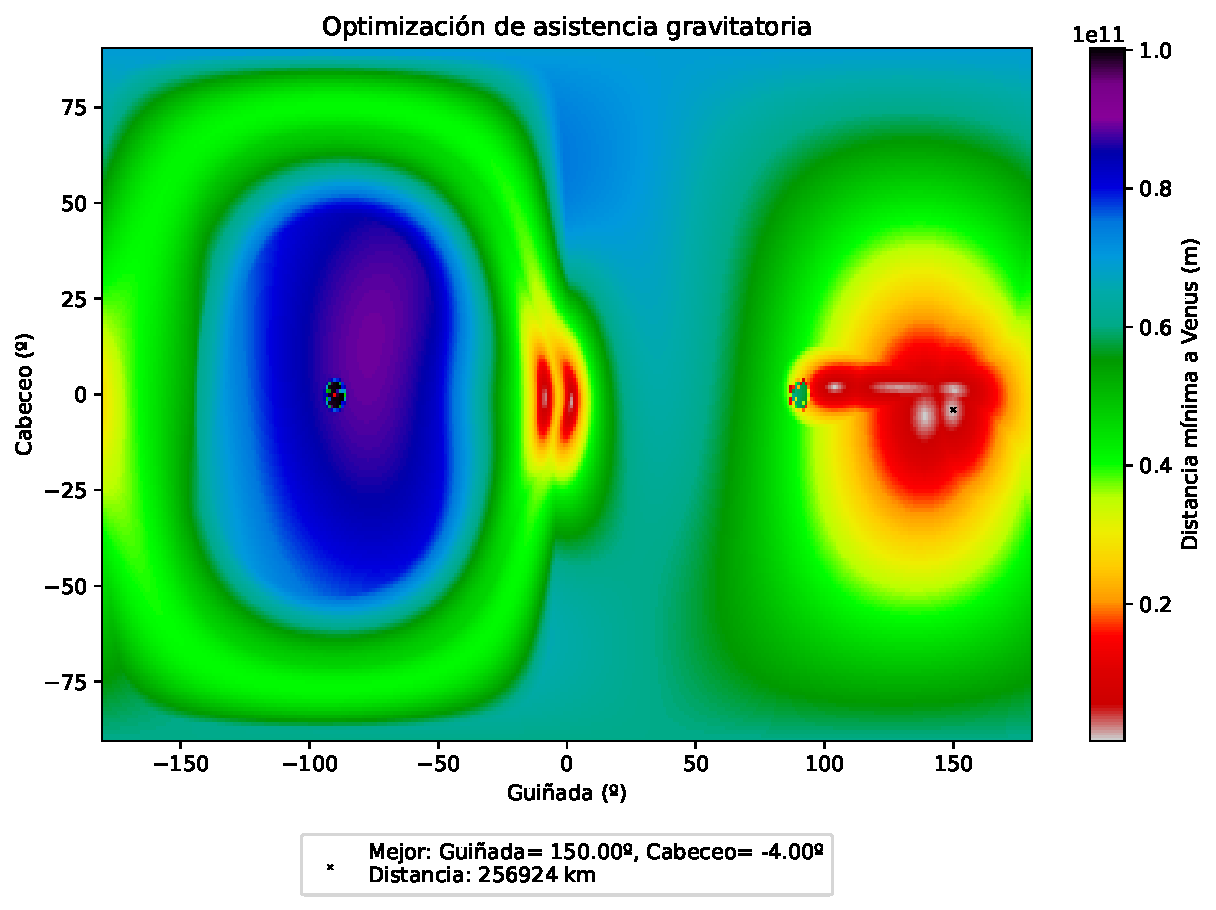
\includegraphics[width=\textwidth]{graphs/heatmap_20260616_162424.pdf}
    % \caption{Mapa de calor que muestra la distancia mínima a Venus en función del ángulo de guiñada y cabeceo.}
\end{figure}
\vspace{-0.5cm}
En él, se pueden apreciar dos principales focos donde la distancia a Venus es pequeña en relación con el resto, 
lo que, como ya ha sido dicho, se corresponde con una mayor transferencia de energía entre Venus y la Nave.
Además, también se pueden observar dos puntos donde ocurren fenómenos extraños; el correspondiente a 
$\sim -100^\circ$ es un choque con la Tierra, y el de $\sim 100^\circ$ con el Sol.
\subsection{Exploración del primer foco}
El primer foco se encuentra ubicado en un entorno de los $0^\circ$ tanto de guiñada como de cabeceo y,
dado que estos valores se corresponden con una velocidad inicial que apunta en la dirección de la de la 
Tierra, se comienza explorando esta zona.
Se realiza entonces un barrido de ángulo de guiñada comprendido en el intervalo $[-20^\circ, +10^\circ]$ y de cabeceo
en $[-15^\circ, +15^\circ]$, con una resolución de $0.25^\circ$. Los parámetros para esta fase son:

\bigskip
\noindent\begin{minipage}{0.5\textwidth}\scriptsize
\begin{verbatim}
double min_yaw_angle = -20.0;
double max_yaw_angle = 10.0;
double min_pitch_angle = -15.0;
double max_pitch_angle = 15.0;
double total_t = 400.0;
double factor = 0.05;
\end{verbatim}
\end{minipage}%
\begin{minipage}{0.5\textwidth}\scriptsize
\begin{verbatim}
double precision_factor = 50.0;
double max_dt = 100;
double min_dt = 0.05;
int pitch_sims = 121;
int yaw_sims = 121;
int total_sims = yaw_sims*pitch_sims;
\end{verbatim}
\end{minipage}

\bigskip

Se obtiene el siguiente gráfico:
\begin{figure}[H]
    \centering
    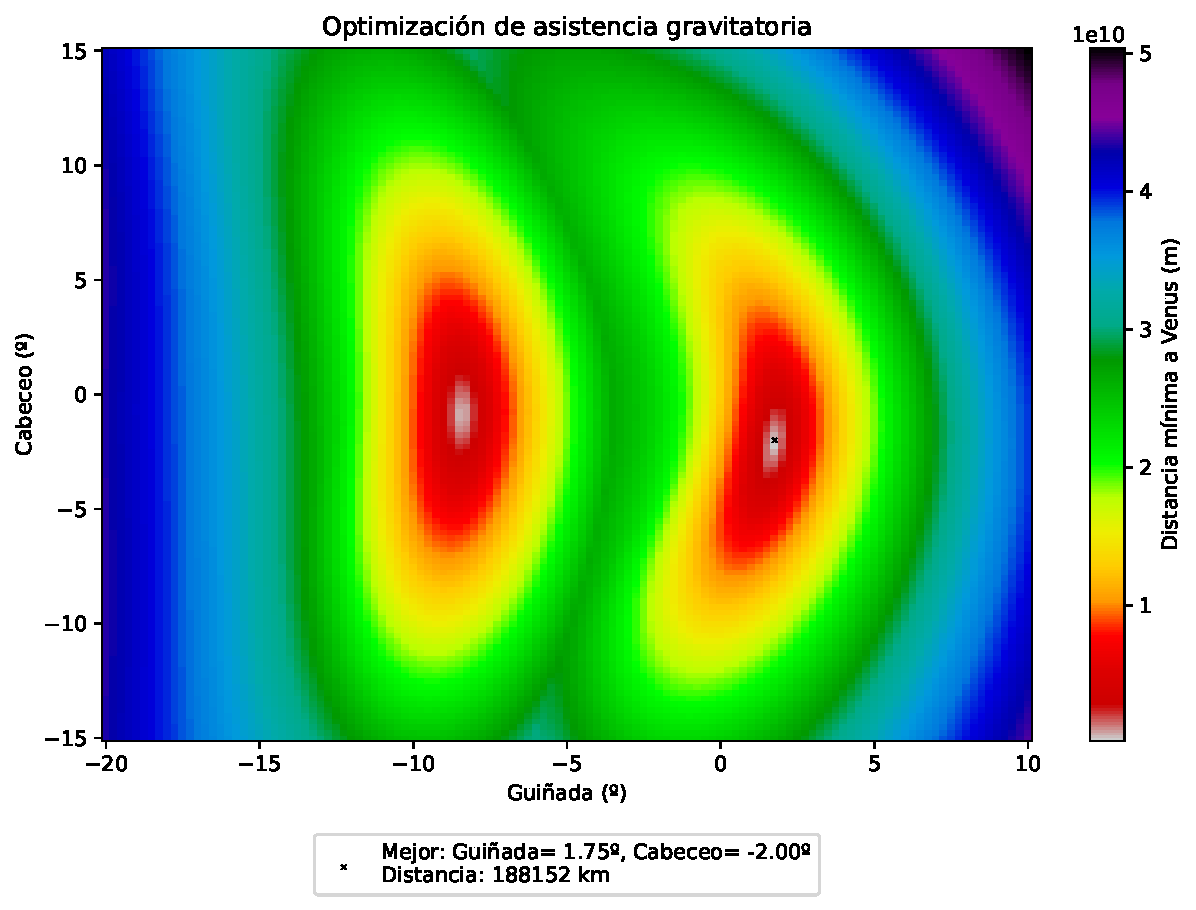
\includegraphics[width=\textwidth]{graphs/heatmap_20260616_164711.pdf}
\end{figure}
Para hilar incluso más fino, se realizará a continuación un análisis centrado en cada una de las dos ventanas:


\subsubsection{Primera ventana}
En primer lugar, se estudia la ventana izquierda, con una resolución de $0.05^\circ$:

\bigskip
\noindent\begin{minipage}{0.5\textwidth}\scriptsize
\begin{verbatim}
double min_yaw_angle = -10.0;
double max_yaw_angle = -6.0;
double min_pitch_angle = -4.0;
double max_pitch_angle = 2.5;
double total_t = 400.0;
double factor = 0.05;
\end{verbatim}
\end{minipage}%
\begin{minipage}{0.5\textwidth}\scriptsize
\begin{verbatim}
double precision_factor = 50.0;
double max_dt = 50;
double min_dt = 0.01;
int pitch_sims = 131;
int yaw_sims = 81;
int total_sims = yaw_sims*pitch_sims;
\end{verbatim}
\end{minipage}

\bigskip

Se obtiene el siguiente resultado:
\begin{figure}[H]
    \centering
    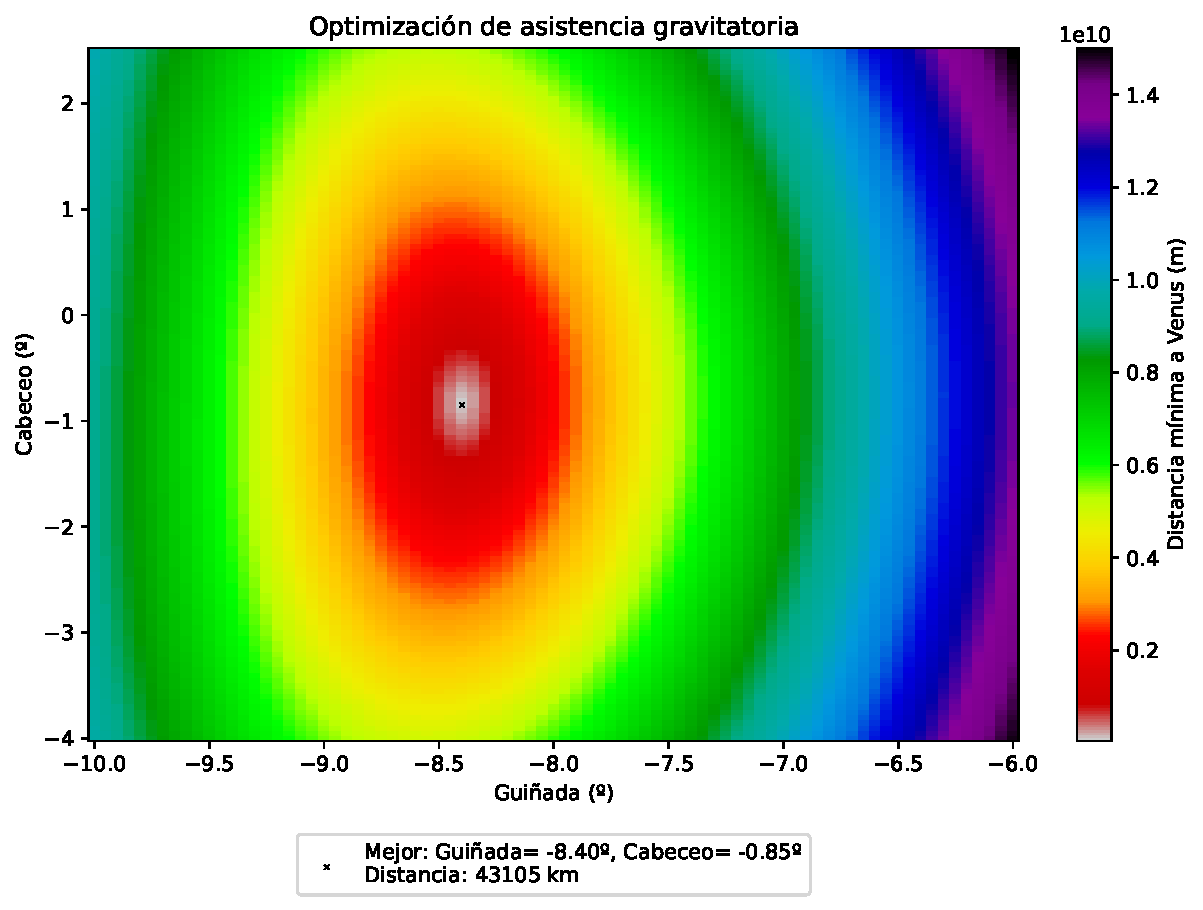
\includegraphics[width=\textwidth]{graphs/heatmap_20260616_170902.pdf}
\end{figure}

Finalmente, para localizar el mínimo con la máxima precisión posible, se realiza un último barrido 
sobre la ventana izquierda, entre $-9^\circ$ y $-8^\circ$ de guiñada y 
entre $-1^\circ$ y $0^\circ$ de cabeceo. 
La resolución se aumenta a $0.005^\circ$, lo que equivale a $18$ segundos de arco. 
Esta configuración resulta en 40401 simulaciones, un número exigente pero asumible.
\newpage
Los parámetros para esta fase final son:

\bigskip
\noindent\begin{minipage}{0.5\textwidth}\scriptsize
\begin{verbatim}
double min_yaw_angle = -9.0;
double max_yaw_angle = -8.0;
double min_pitch_angle = -1.0;
double max_pitch_angle = 0.0;
double total_t = 400.0;
double factor = 0.05;
\end{verbatim}
\end{minipage}%
\begin{minipage}{0.5\textwidth}\scriptsize
\begin{verbatim}
double precision_factor = 50.0;
double max_dt = 50;
double min_dt = 0.01;
int pitch_sims = 201;
int yaw_sims = 201;
int total_sims = yaw_sims*pitch_sims;
\end{verbatim}
\end{minipage}

\bigskip

\begin{figure}[H]
    \centering
    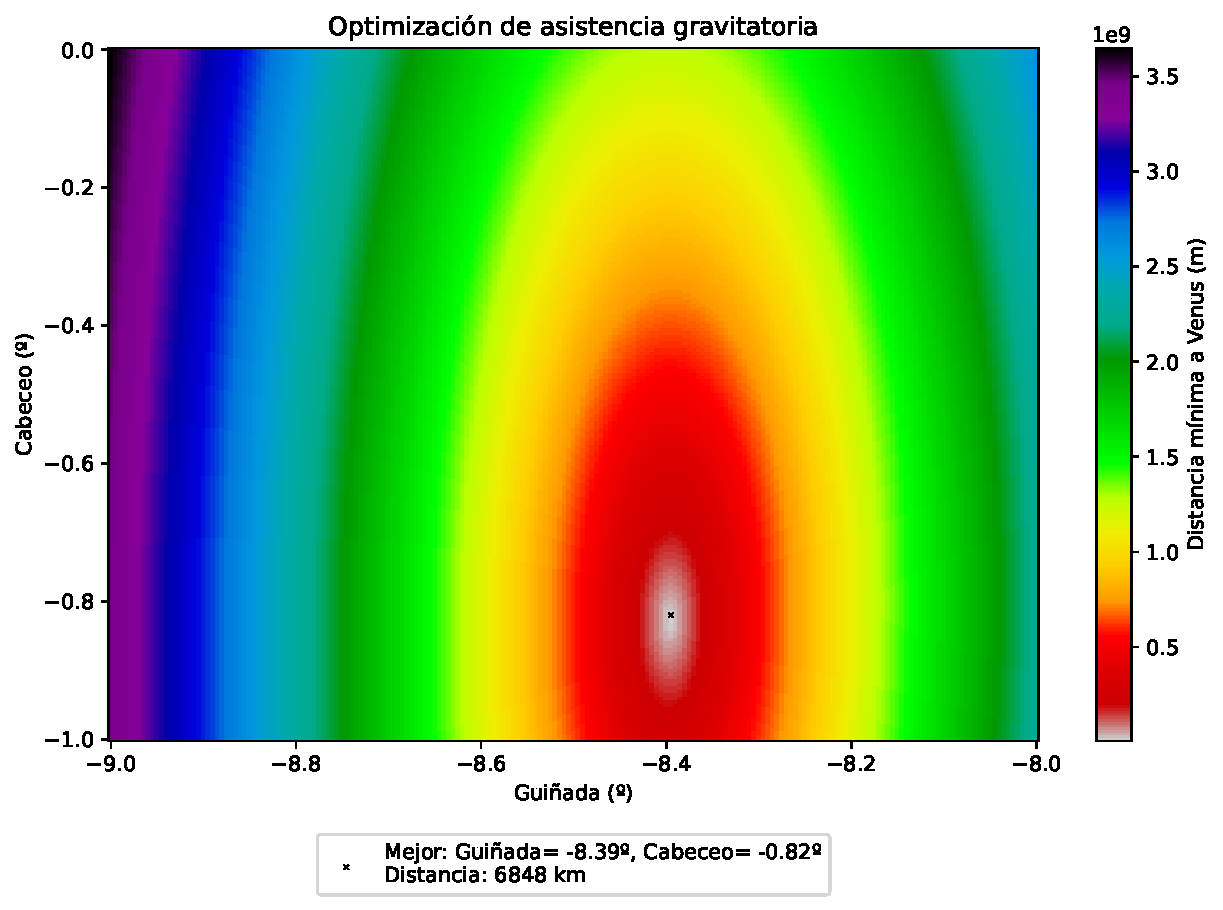
\includegraphics[width=\textwidth]{graphs/heatmap_20260616_181013.pdf}
\end{figure}
Los ángulos óptimos obtenidos son:
\begin{itemize}
    \item Guiñada, $\varphi = -8.39500^\circ$
    \item Cabeceo, $\theta = -0.82000^\circ$
\end{itemize}


\newpage
\subsubsection{Segunda ventana}
A continuación, se explora la segunda ventana de interés, con una resolución de $0.05^\circ$. El barrido se realiza en el intervalo de guiñada $[0^\circ, 4^\circ]$ y de cabeceo $[-4.5^\circ, 2^\circ]$.
Los parámetros para esta fase son:

\bigskip
\noindent\begin{minipage}{0.5\textwidth}\scriptsize
\begin{verbatim}
double min_yaw_angle = 0.0;
double max_yaw_angle = 4.0;
double min_pitch_angle = -4.5;
double max_pitch_angle = 2.0;
double total_t = 400.0;
double factor = 0.05;
\end{verbatim}
\end{minipage}%
\begin{minipage}{0.5\textwidth}\scriptsize
\begin{verbatim}
double precision_factor = 50.0;
double max_dt = 50;
double min_dt = 0.01;
int pitch_sims = 131;
int yaw_sims = 81;
int total_sims = yaw_sims*pitch_sims;
\end{verbatim}
\end{minipage}

\bigskip

\begin{figure}[H]
    \centering
    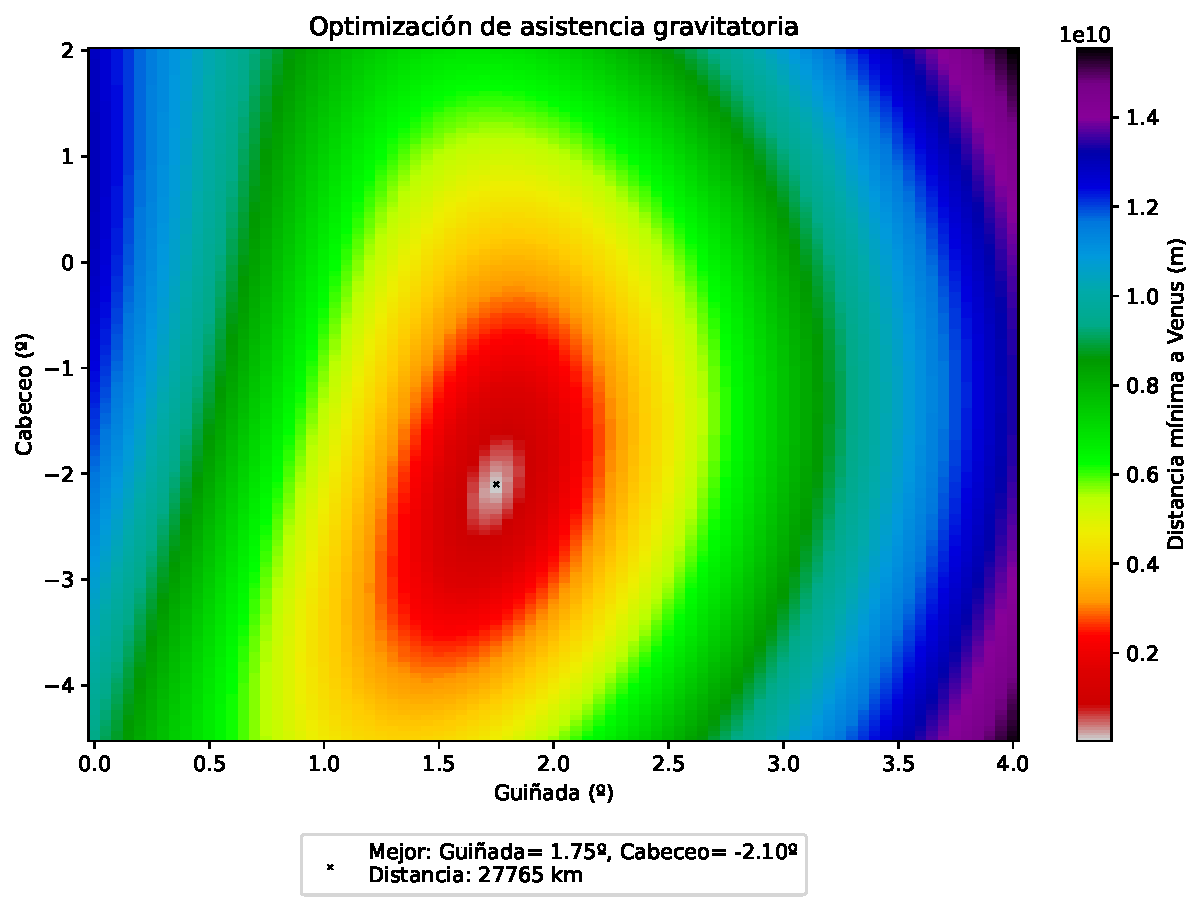
\includegraphics[width=\textwidth]{graphs/heatmap_20260616_182644.pdf}
\end{figure}


\bigskip

De nuevo, para localizar el mínimo con la máxima precisión posible, se realiza un último barrido 
sobre esta segunda ventana, entre $1.5^\circ$ y $2^\circ$ de guiñada y 
entre $-2.3^\circ$ y $-1.8^\circ$ de cabeceo. 
La resolución se mantiene en $0.005^\circ$ (18 segundos de arco). 
Esta configuración resulta en 10201 simulaciones.
\newpage
Los parámetros para esta fase final son:

\bigskip
\noindent\begin{minipage}{0.5\textwidth}\scriptsize
\begin{verbatim}
double min_yaw_angle = 1.5;
double max_yaw_angle = 2.0;
double min_pitch_angle = -2.3;
double max_pitch_angle = -1.8;
double total_t = 400.0;
double factor = 0.05;
\end{verbatim}
\end{minipage}%
\begin{minipage}{0.5\textwidth}\scriptsize
\begin{verbatim}
double precision_factor = 50.0;
double max_dt = 50;
double min_dt = 0.01;
int pitch_sims = 101;
int yaw_sims = 101;
int total_sims = yaw_sims*pitch_sims;
\end{verbatim}
\end{minipage}
\bigskip

\begin{figure}[H]
    \centering
    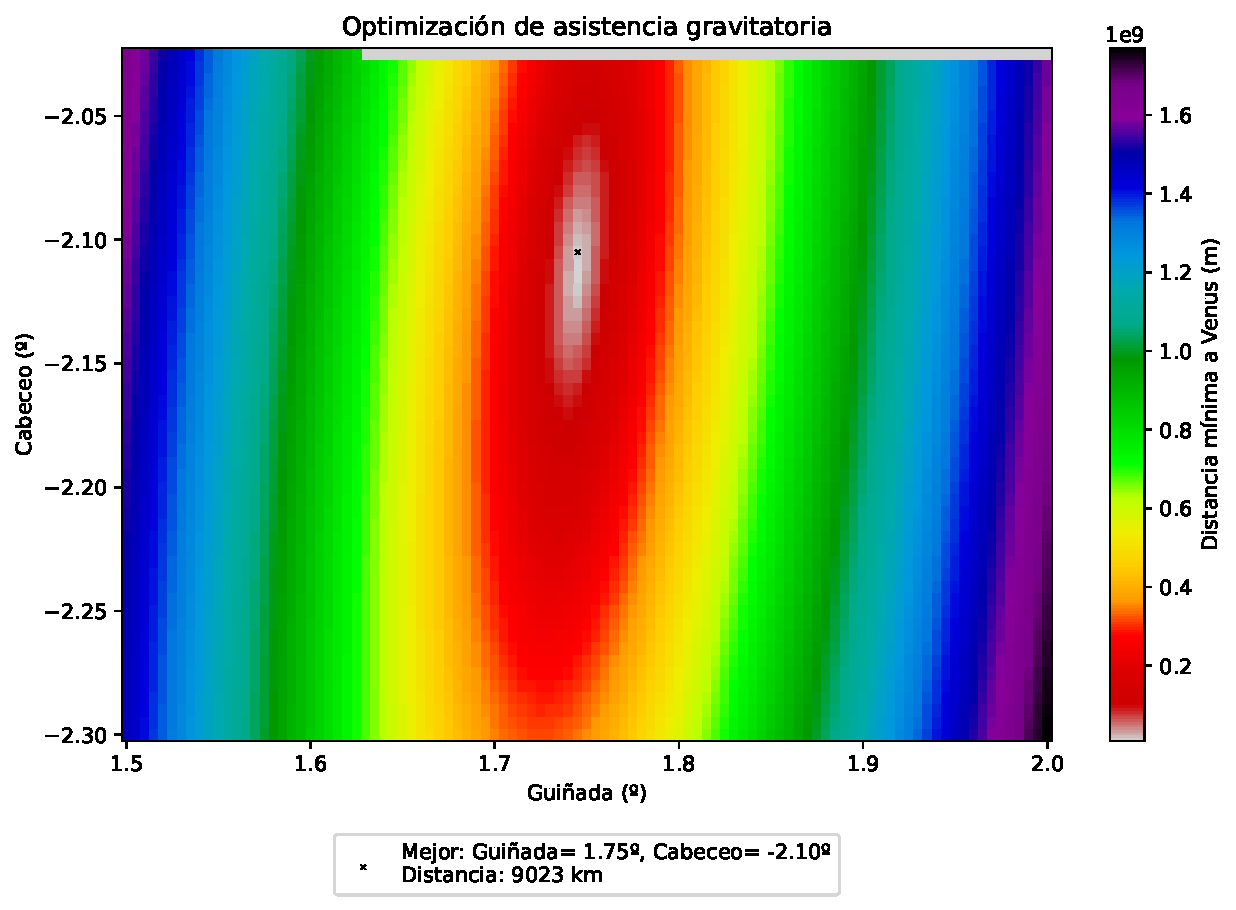
\includegraphics[width=\textwidth]{graphs/heatmap_20260616_184803.pdf}
\end{figure}
Los ángulos óptimos obtenidos son:
\begin{itemize}
    \item Guiñada, $\varphi = 1.74500^\circ$
    \item Cabeceo, $\theta = -2.10500^\circ$
\end{itemize}
\section{Análisis de las Trayectorias Óptimas}
Una vez identificados los ángulos de lanzamiento que minimizan la distancia de aproximación a Venus, se procede a analizar en detalle las trayectorias correspondientes a los dos puntos óptimos encontrados en las dos ventanas de interés.

\subsection{Primer Punto Óptimo (Ventana 1)}
Este punto, con ángulos de Guiñada $\varphi = -8.395^\circ$ y Cabeceo $\theta = -0.820^\circ$, corresponde a una maniobra que resulta en una \textbf{pérdida de energía} de la nave, cumpliendo el objetivo de acercarse al Sol.

\begin{figure}[H]
    \centering
    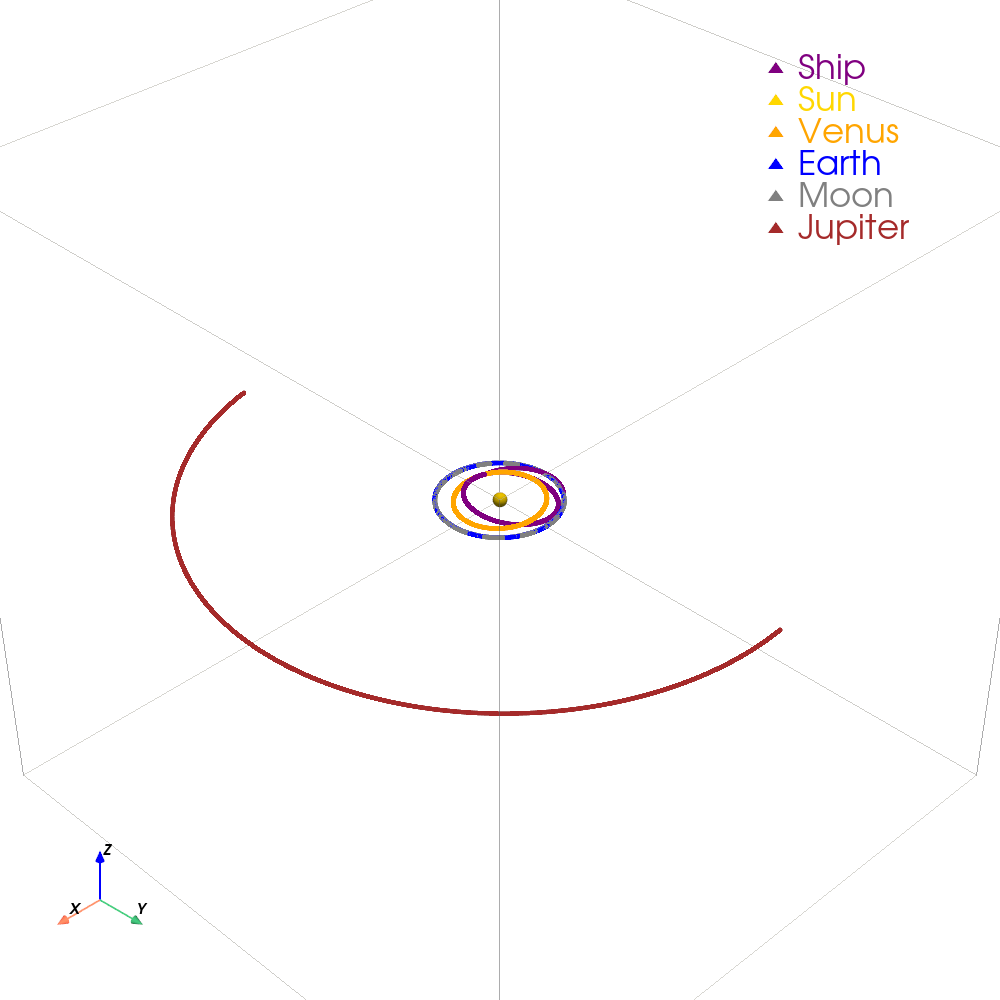
\includegraphics[width=0.8\textwidth]{graphs/acercamiento/orbit_plot_1.png}
    \caption{Trayectoria 3D de la simulación óptima (acercamiento).}
\end{figure}

\begin{figure}[H]
    \centering
    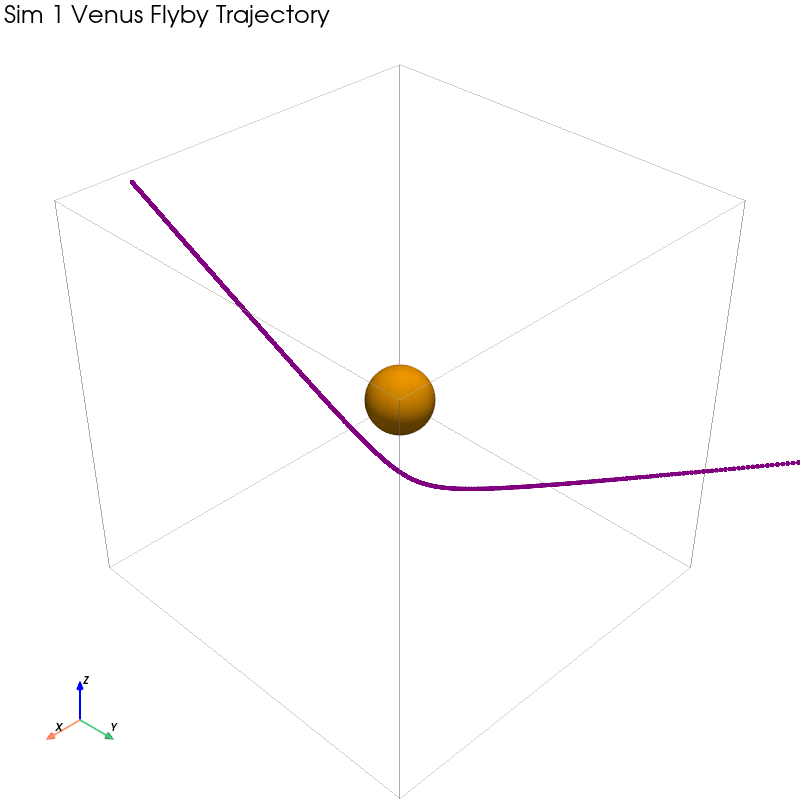
\includegraphics[width=0.5\textwidth]{graphs/acercamiento/venus_flyby_static_1.png}
    \caption{Detalle de la trayectoria hiperbólica durante el sobrevuelo de Venus (acercamiento).}
\end{figure}

\begin{figure}[H]
    \centering
    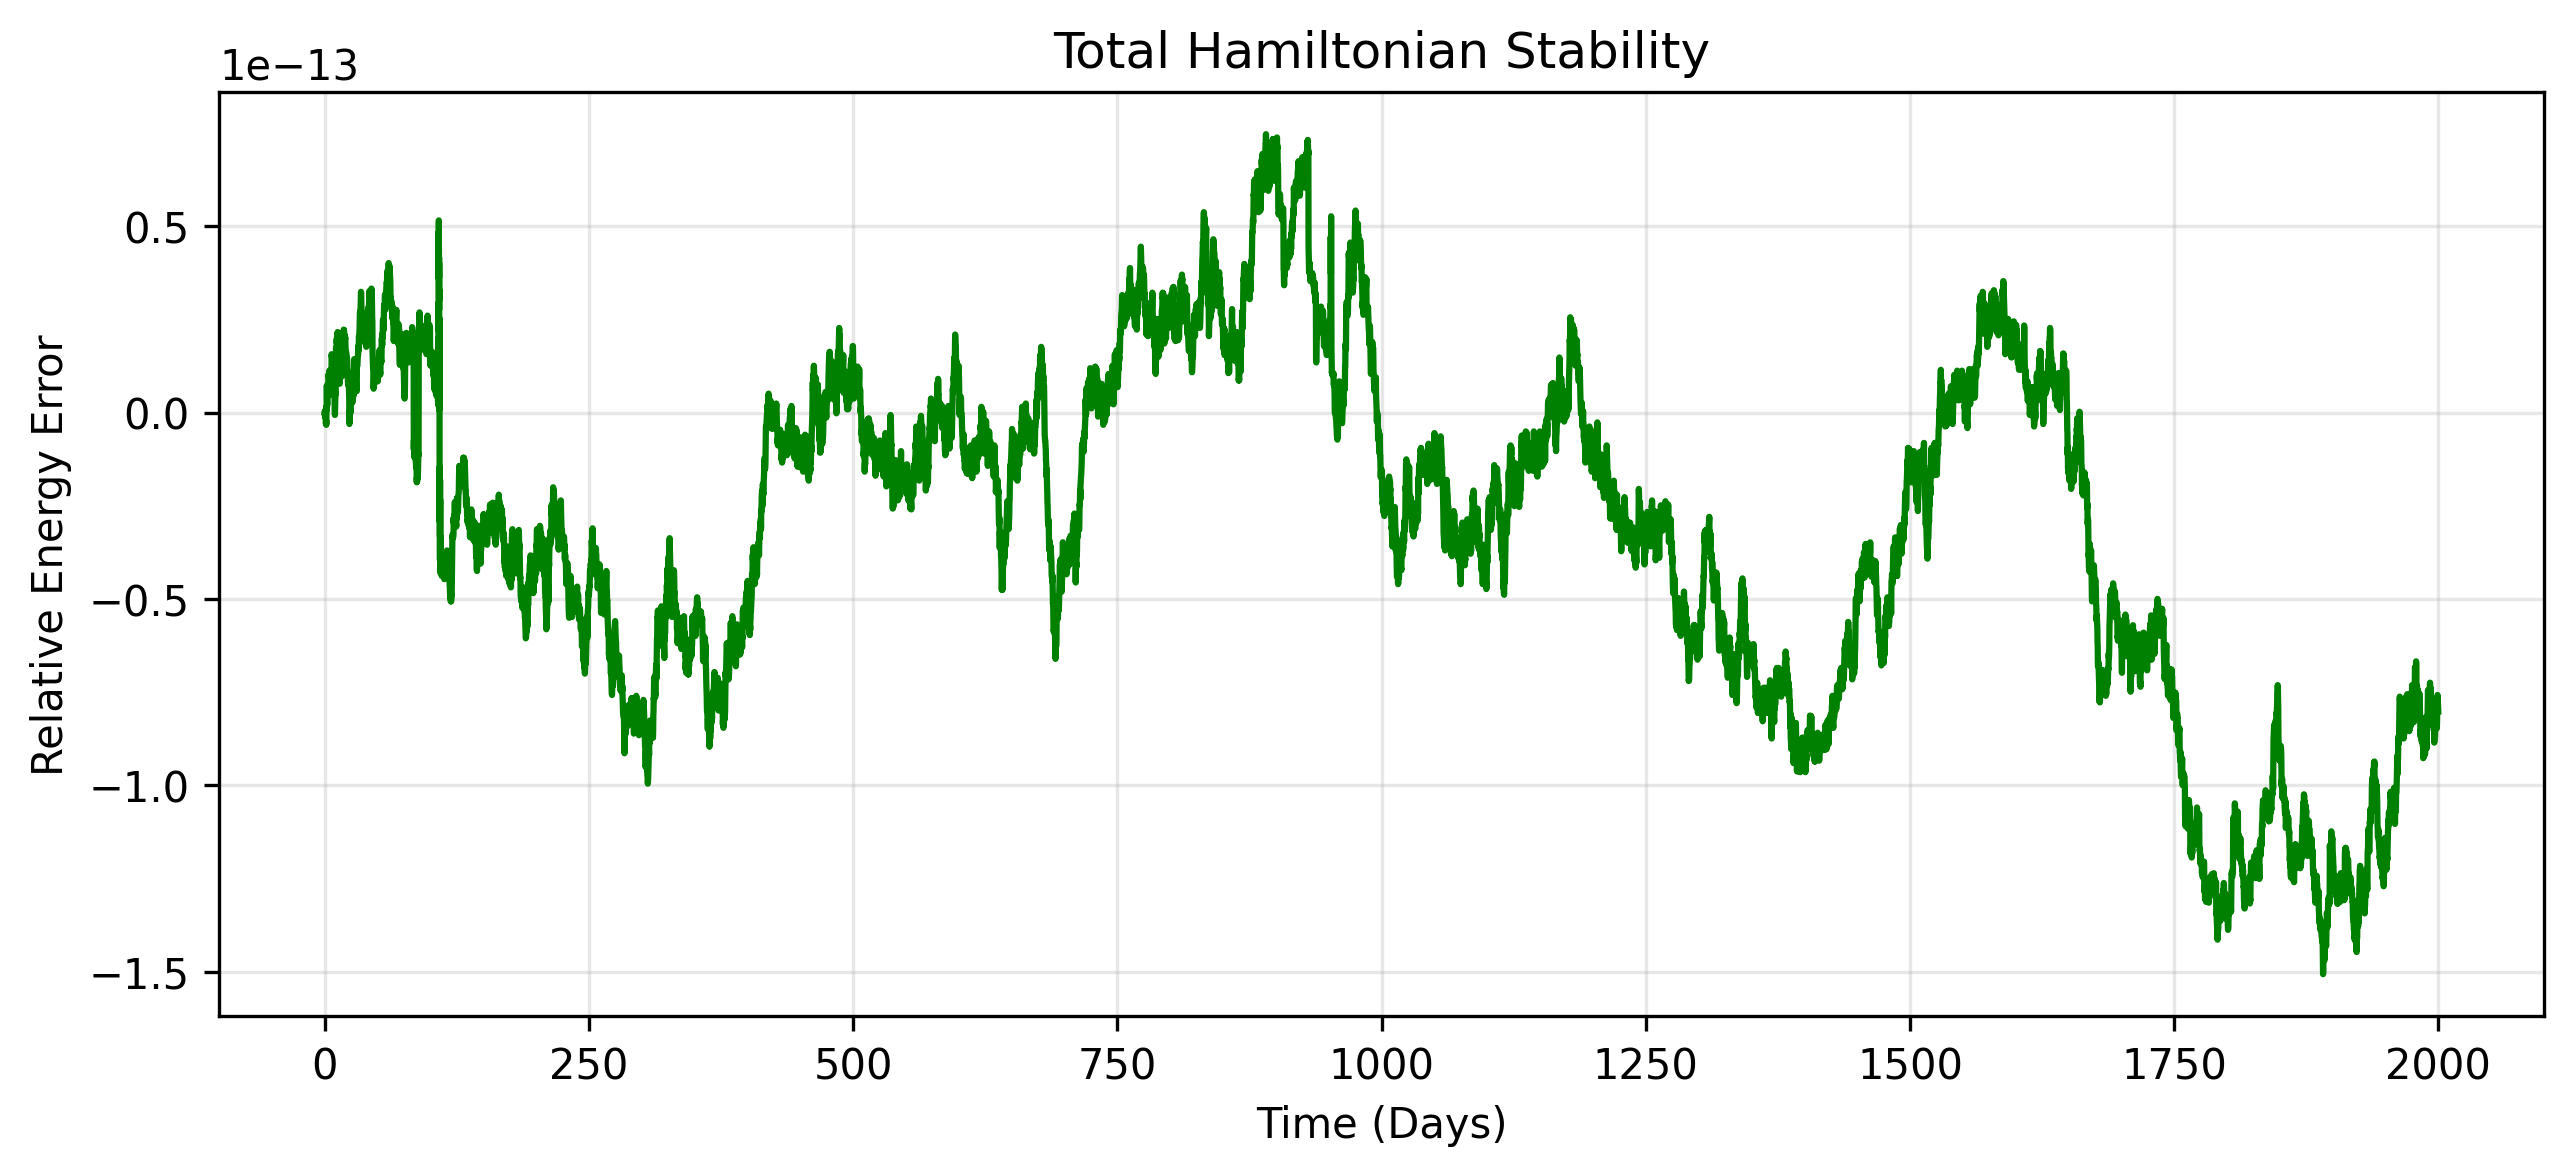
\includegraphics[width=0.8\textwidth]{graphs/acercamiento/total_energy_1.png}
    \caption{Error relativo de la energía total del sistema (acercamiento).}
\end{figure}

\begin{figure}[H]
    \centering
    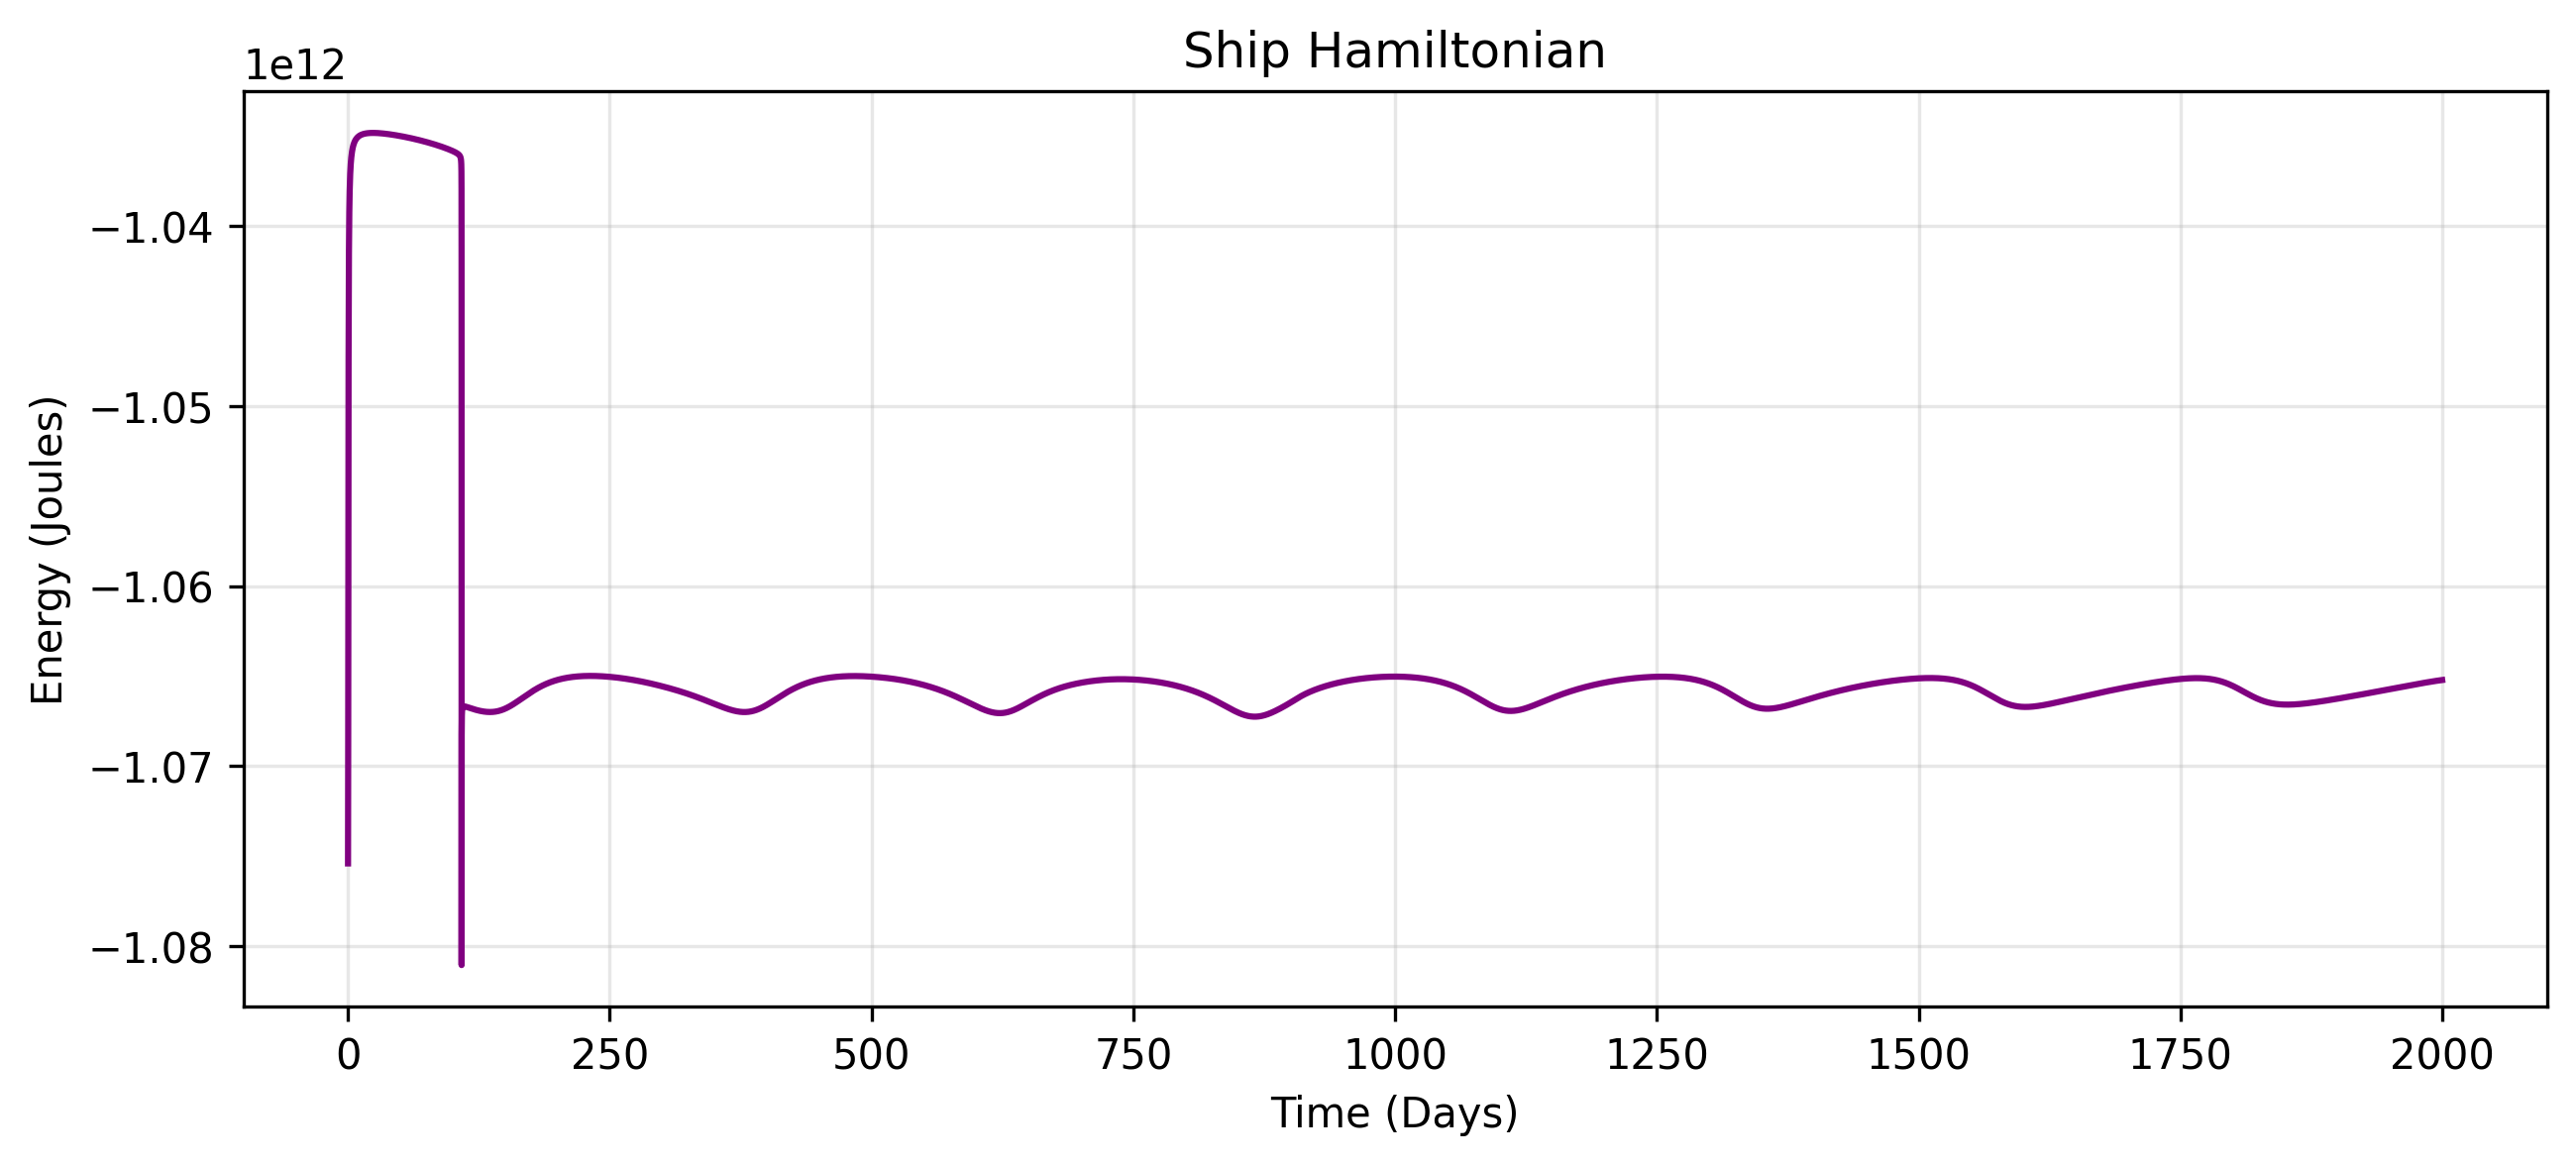
\includegraphics[width=0.8\textwidth]{graphs/acercamiento/ship_energy_1.png}
    \caption{Energía específica de la nave (acercamiento). Se observa un salto energético negativo ($\Delta E \approx -2.9 \cdot 10^{10}$ J) tras el encuentro con Venus, así como un pequeño bug al inicio.}
\end{figure}

\subsection{Segundo Punto Óptimo (Ventana 2)}
Este segundo punto, con ángulos de Guiñada $\varphi = 1.745^\circ$ y Cabeceo $\theta = -2.105^\circ$, corresponde a una maniobra que resulta en una \textbf{ganancia de energía} de la nave. Aunque no cumple el objetivo principal, es un resultado físicamente interesante.

\begin{figure}[H]
    \centering
    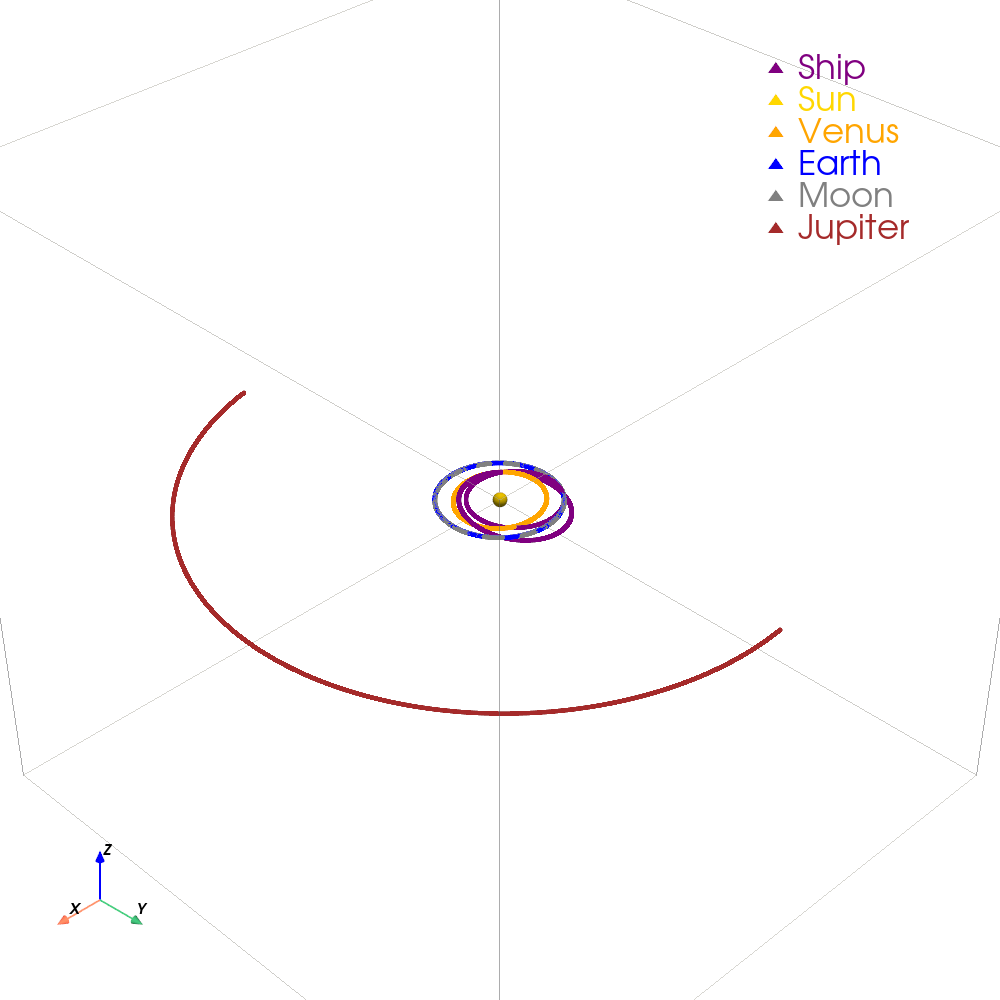
\includegraphics[width=0.8\textwidth]{graphs/alejamiento/orbit_plot_1.png}
    \caption{Trayectoria 3D de la simulación óptima (alejamiento).}
\end{figure}

\begin{figure}[H]
    \centering
    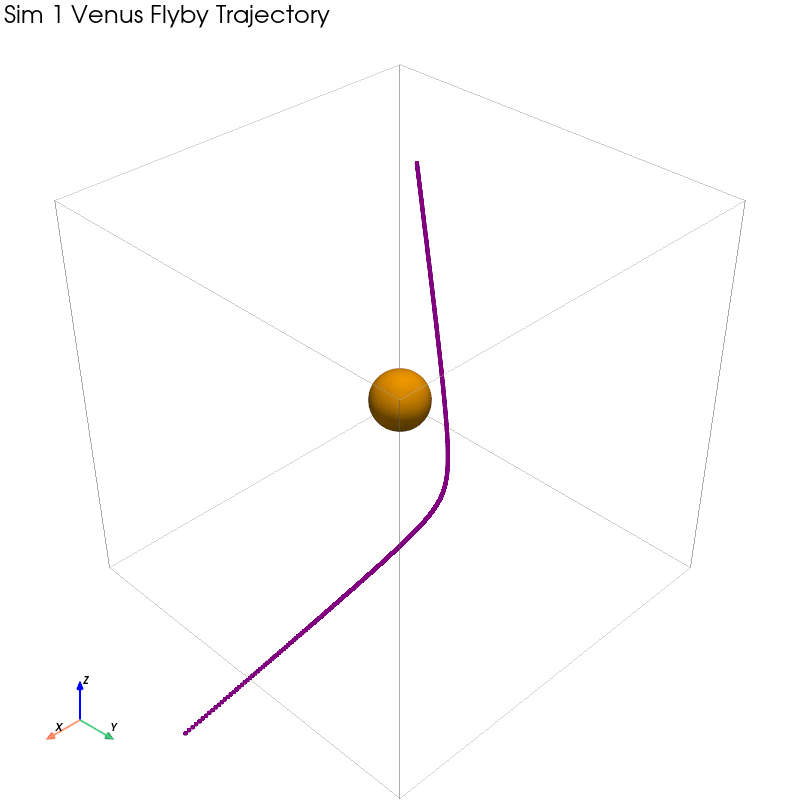
\includegraphics[width=0.5\textwidth]{graphs/alejamiento/venus_flyby_static_1.png}
    \caption{Detalle de la trayectoria hiperbólica durante el sobrevuelo de Venus (alejamiento).}
\end{figure}

\begin{figure}[H]
    \centering
    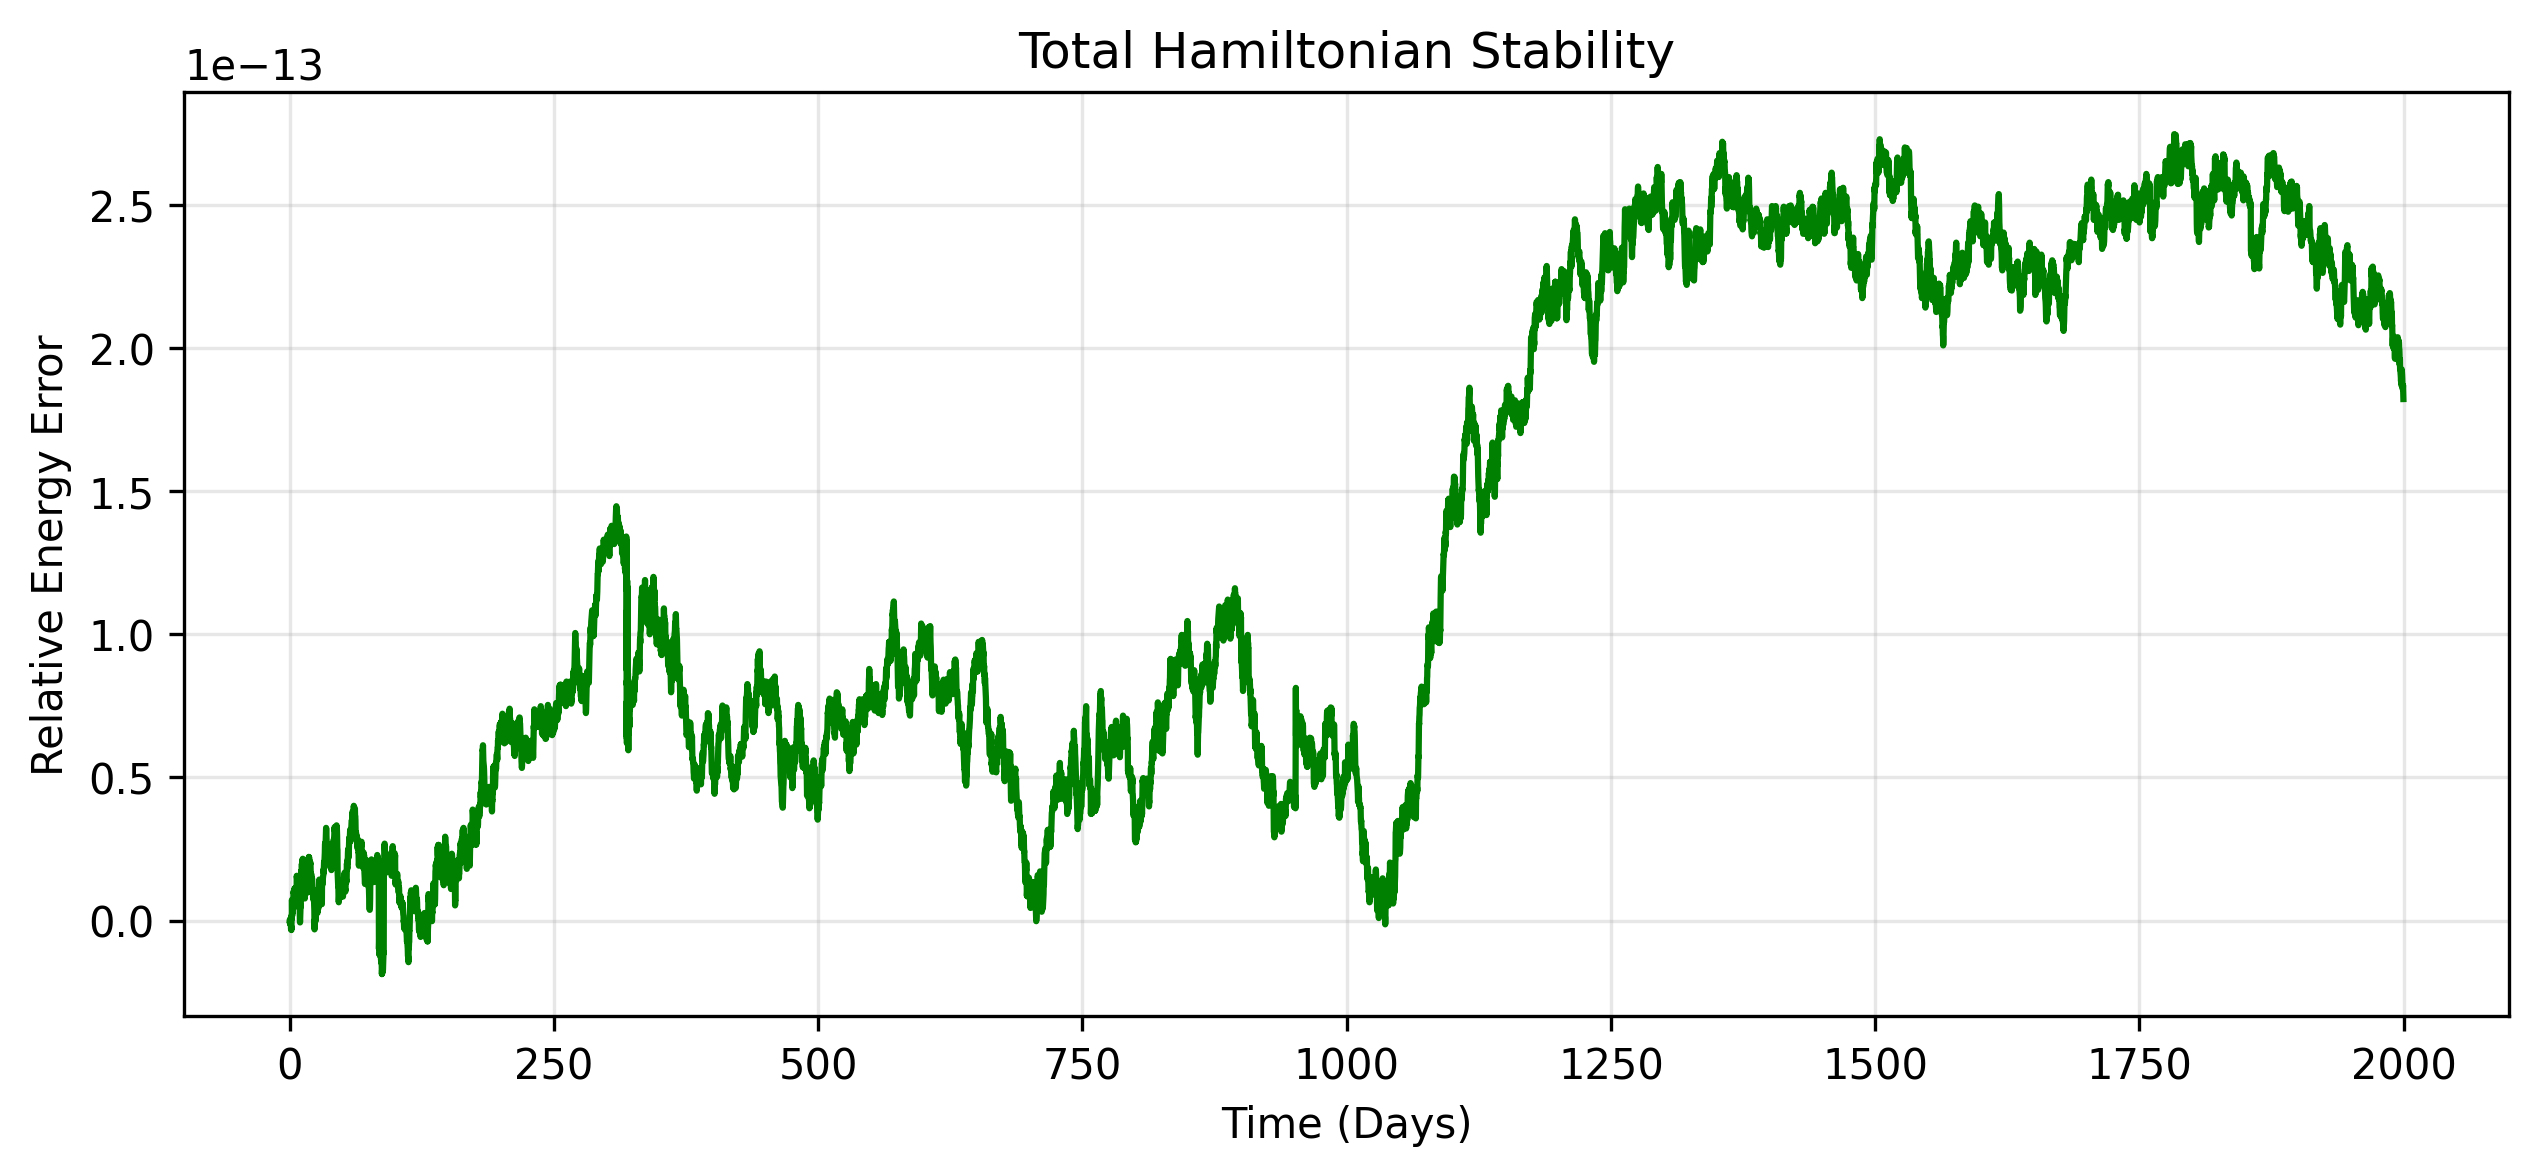
\includegraphics[width=0.8\textwidth]{graphs/alejamiento/total_energy_1.png}
    \caption{Error relativo de la energía total del sistema (alejamiento).}
\end{figure}

\begin{figure}[H]
    \centering
    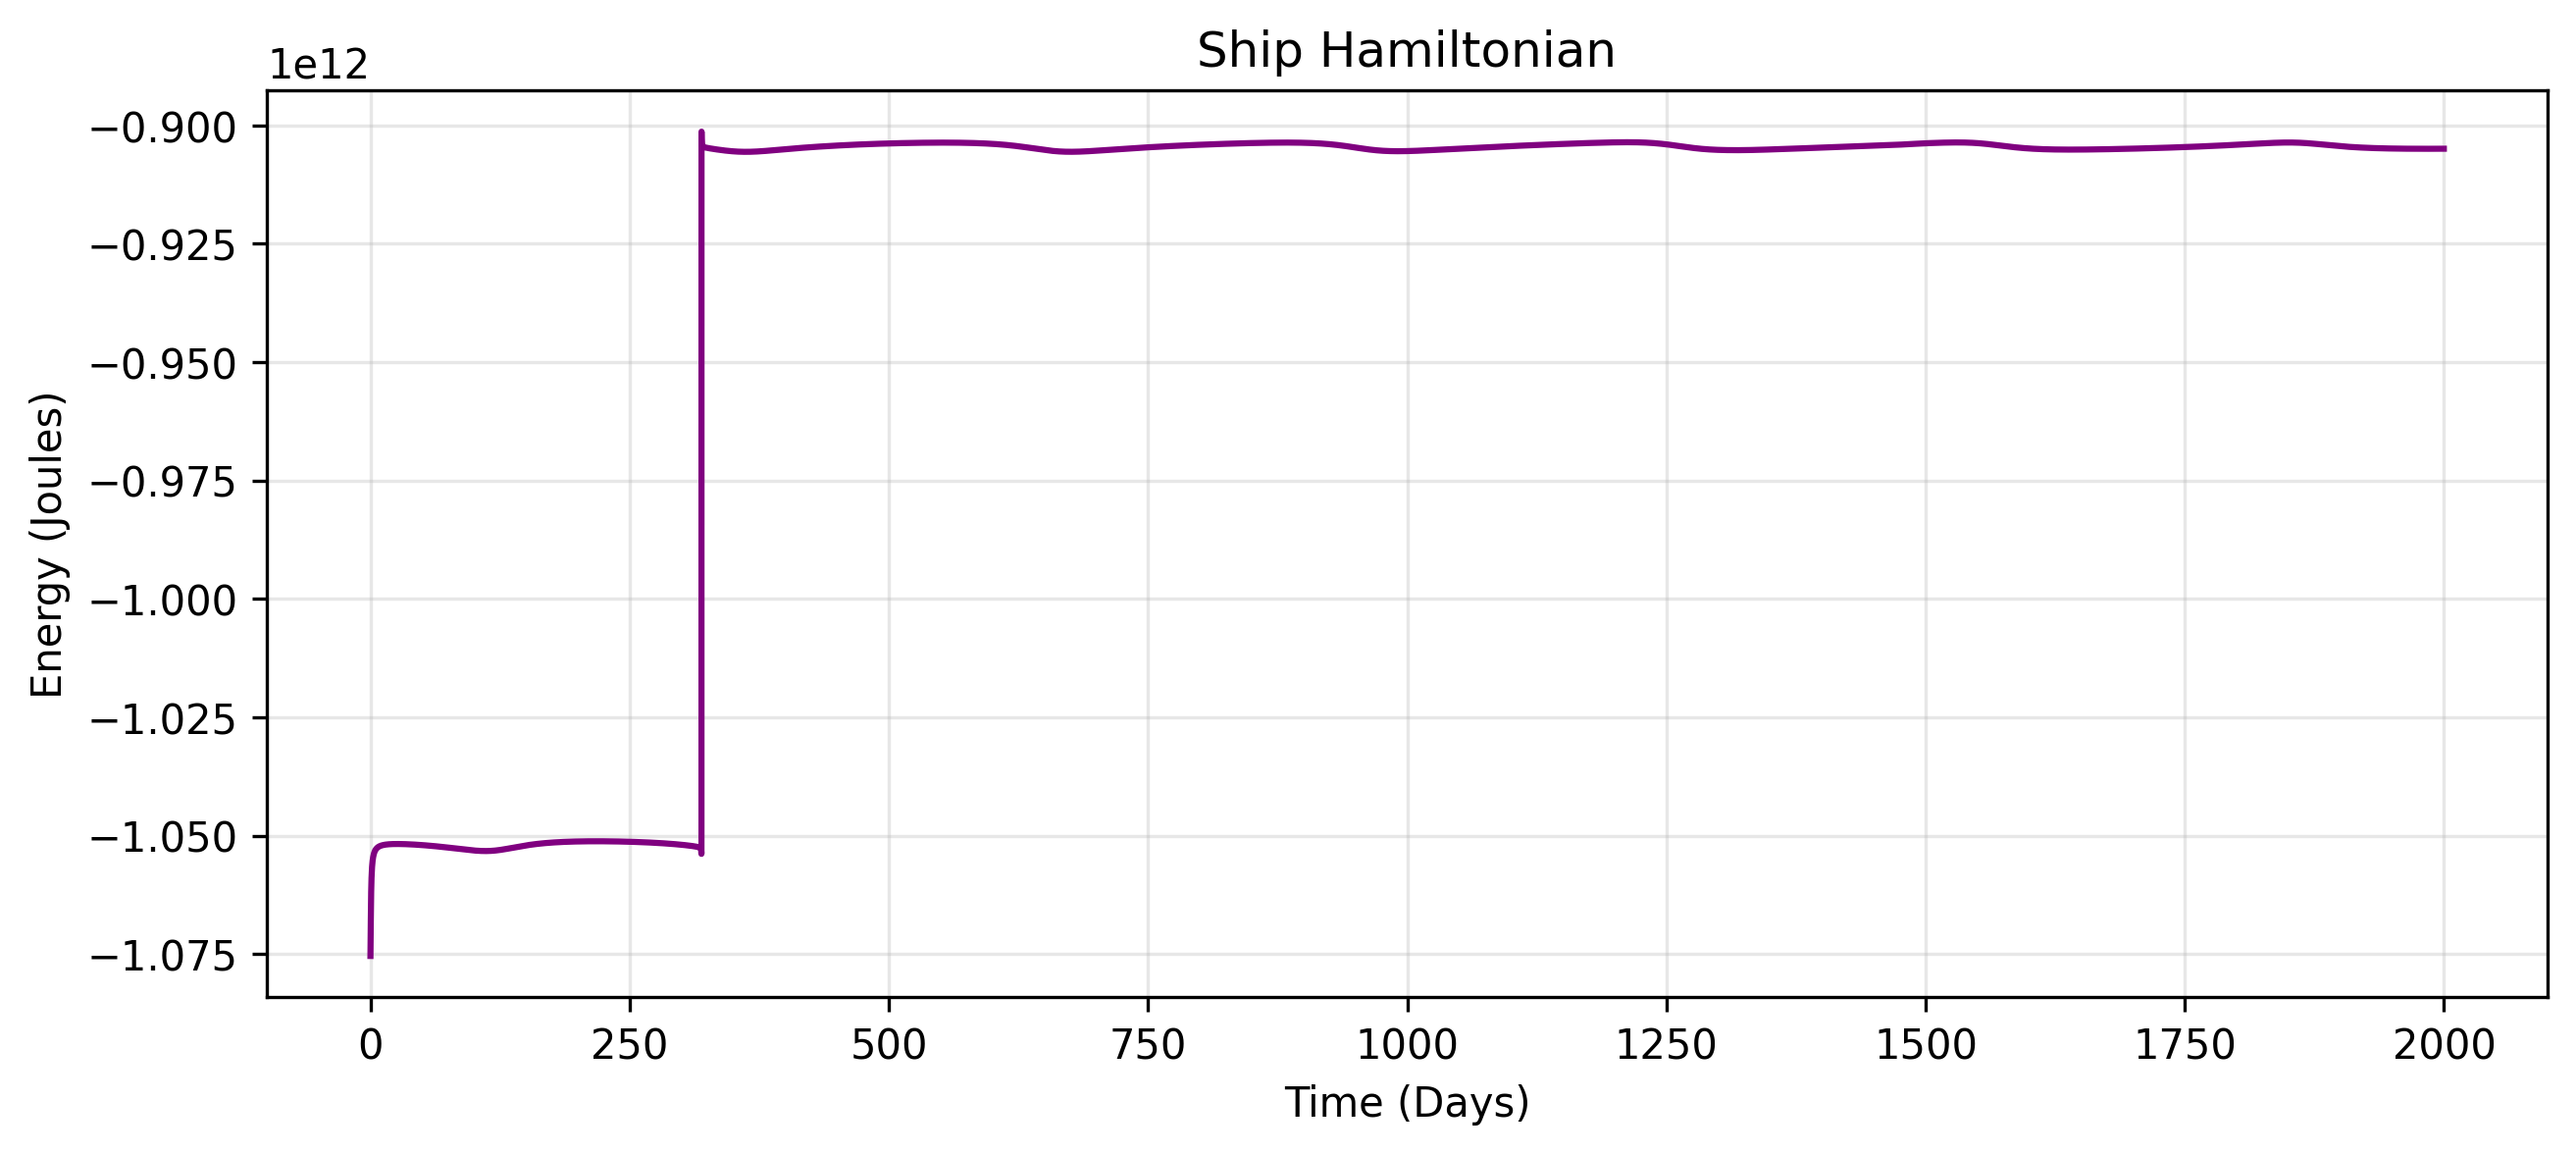
\includegraphics[width=0.8\textwidth]{graphs/alejamiento/ship_energy_1.png}
    \caption{Energía específica de la nave (alejamiento). Se observa un salto energético positivo ($\Delta E \approx +1.7 \cdot 10^{11}$ J) tras el encuentro con Venus.}
\end{figure}

\subsection{Vídeos y HTML Interactivo}
Adicionalmente, se han generado vídeos de la simulación completa y de la maniobra de aproximación a Venus, 
así como un \textit{html} interactivo de la órbita tridimensional en el Sistema Solar, que se pueden 
encontrar tanto en la carpeta de resultados adjunta como en el GitHub.
\section{Conclusiones}
En este trabajo, se ha abordado el complejo problema de la simulación de una maniobra de asistencia gravitatoria, 
un pilar fundamental de la astrodinámica moderna; para ello, se ha desarrollado desde cero un 
simulador del Sistema Solar en C, utilizando un integrador Runge-Kutta de cuarto orden con paso de tiempo adaptativo, 
lo que ha permitido obtener un equilibrio muy bueno, creo yo, entre precisión numérica y coste computacional.

El objetivo principal, que era encontrar los ángulos de lanzamiento óptimos para que una sonda, 
con condiciones iniciales inspiradas en la misión Solar Orbiter, maximizara la transferencia de energía con 
Venus, se ha logrado con éxito; mediante un sistema de barrido de parámetros orquestado por Python y ejecutado por C, 
se ha podido explorar sistemáticamente el espacio de soluciones, identificando no una, sino dos familias de 
trayectorias óptimas.

Este proceso de optimización, que se ha llevado a cabo en varias fases, primero con un barrido grueso 
para mapear todo el espacio de posibilidades, y luego con sucesivos barridos finos de resolución creciente, 
ha demostrado ser una estrategia muy potente; ha permitido, de hecho, localizar con una precisión de hasta 0.005 
grados los ángulos de guiñada y cabeceo que minimizan la distancia de aproximación al planeta, que, como se demostró 
en la introducción, es la clave para una asistencia gravitatoria efectiva.

Los resultados, además, son físicamente muy interesantes; se ha encontrado una trayectoria que, efectivamente, 
pierde energía al interactuar con Venus, cumpliendo el objetivo de "frenar" para acercarse al Sol
($\Delta E \approx -2.9 \cdot 10^{10}$ J), pero también 
se ha identificado otra que, por el contrario, gana energía, alejándose (con un $\Delta E \approx +1.7 \cdot 10^{11}$ J). 
El análisis de las gráficas de energía de la nave confirma, de forma visual e inequívoca, estos saltos energéticos 
justo en el momento del sobrevuelo; mientras que la conservación de la energía total del sistema, con un error 
relativo del orden de $10^{-14}$, valida la robustez y estabilidad del integrador numérico implementado.

No obstante, este trabajo, como todo modelo, posee sus limitaciones inherentes; la ausencia de propulsión activa 
en la nave, la simplificación de la atmósfera de Venus a un umbral de colisión, o la no consideración de perturbaciones 
gravitatorias de cuerpos menores, son factores que, sin duda, podrían refinarse en futuras investigaciones; 
abriendo, así, nuevas vías para explorar optimizaciones multi-objetivo o, incluso, el diseño de complejas 
cadenas de asistencias gravitatorias, que es un campo, por cierto, apasionante y que pensaba explorar con este 
trabajo, pero no me ha sido posible.

En definitiva, se ha construido una herramienta de simulación y análisis muy completa, que no solo ha 
permitido recrear un fenómeno físico complejo con gran fidelidad, sino que también ha servido para aplicar 
y visualizar conceptos fundamentales de la mecánica clásica, como son los problemas de dispersión, la importancia de las condiciones iniciales para evitar trayectorias catastróficas, y la 
conservación de la energía y el momento angular, todo ello, además, con un resultado que, visualmente, es 
bastante espectacular.

\end{document}